\newpage
\chapter{Background}
\label{ch:background}

% \color{gray}
% \todo{Überleitung wenn Einleitung da ist}
% \section{Iron Reduction}
% In this master thesis we look at iron as a
% carbon-free energy carrier in a reduction-oxidation cycle. Reducing iron oxide can be done via hydrogen for which several industrial-scale technologies exist such as the steam-iron redox process \cite{coalToIron}. 
% For this cycle iron oxide is reduced
% \begin{align*}
%     \ce{Fe2O3 + 3H2 -> 2Fe + 3H2O}
% \end{align*}
% which is an endothermic process. The stored iron is then oxidized to iron oxide which is a exothermic process. 
% As the efficiency of the iron storage cycle depends on the efficiency of both the oxidation and the reduction step both need to be as efficient as possible.
% The goal of this master thesis is a numerical simulation of a simplified reduction in a fluidized bed reactor.


% Classification of the particle: Fall in category C, difficult to fluidize lots of forces in between the particles.
% \todo{Noch nicht fertig}










% \section{Fluidized Bed Reactor}
% \label{sec:basicFBR}

% Fluidized Bed Reactors (FBR) are a cornerstone of multiphase chemical processing, with recent experimental studies highlighting their efficacy in the reduction of iron oxide \cite{Malte}. In a typical setup, solid particles are loaded into a reactor vessel, resting atop a porous distributor plate. This accumulation of solids is referred to as the particle bed.

% The fundamental principle of an FBR is the suspension of these solid particles by an upward-flowing fluid—in this study, a gas. This suspension induces fluid-like properties in the granular material, such as the ability of lighter objects to float on the bed surface and the maintenance of a horizontal surface level even when the reactor is tilted \cite{zustand_eng}.

% \subsection{Fluidization Regimes}
% The behavior of the bed is strictly dependent on the superficial gas velocity. Figure \ref{fig:fluidize_states} illustrates the progression of fluidization regimes:

% \begin{enumerate}
%     \item \textbf{Fixed Bed:} At low inflow rates, the gas percolates through the interstitial spaces between stationary particles. The drag force is insufficient to overcome gravity, and the bed remains static.
%     \item \textbf{Minimum Fluidization:} As the inflow velocity approaches the minimum fluidization velocity, denoted as $u_{mf}$, the upward drag force ($F_D$) equilibrates with the gravitational force ($F_g$) acting on the particles. At this point, the bed begins to expand and particles are suspended.
%     \item \textbf{Bubbling Fluidization:} As the velocity exceeds $u_{mf}$, the bed expands further. In gas-solid systems, instabilities arise, leading to the formation of voids or "bubbles" near the distributor plate. These bubbles coalesce as they rise, promoting vigorous mixing.
%     \item \textbf{Turbulent Fluidization and Pneumatic Transport:} At significantly higher velocities, the distinct upper surface of the bed vanishes, and the particle motion becomes turbulent. Eventually, the drag force is sufficient to entrain solids out of the reactor entirely, a state known as pneumatic transport.
% \end{enumerate}

% \begin{figure}[h!]
%     \centering
%     % Improved spacing: using subfigure or minipage is often safer, 
%     % but standard includegraphics with width fractions works if sums < 1.0
%     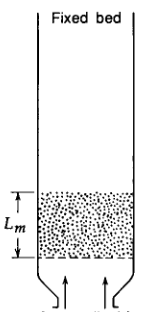
\includegraphics[width=0.23\linewidth, keepaspectratio]{sections/background/FixedBed.png}
%     \hfill
%     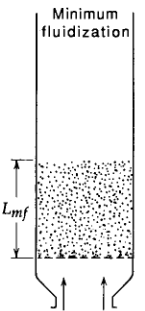
\includegraphics[width=0.23\linewidth, keepaspectratio]{sections/background/MinimumFluidization.png}
%     \hfill
%     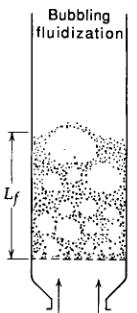
\includegraphics[width=0.23\linewidth, keepaspectratio]{sections/background/BubblingFluidization.png}
%     \hfill
%     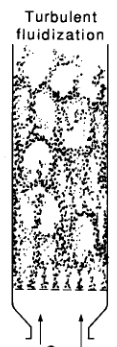
\includegraphics[width=0.23\linewidth, keepaspectratio]{sections/background/TrubulentFluidization.png}
%     \caption{Fluidization states for increasing inflow velocities (left to right): Fixed Bed, Minimum Fluidization, Bubbling Fluidization, and Turbulent Fluidization. Adapted from \cite{zustand_eng}.}
%     \label{fig:fluidize_states}
% \end{figure}

% \subsection{Pressure Drop Mechanics}
% A key physical indicator of fluidization is the pressure drop across the bed, $\Delta p$. 
% In the fixed bed regime ($u < u_{mf}$), the pressure drop increases practically linearly with gas velocity. 
% However, once the bed is fluidized ($u \geq u_{mf}$), the pressure drop plateaus. This occurs because the drag force supports the full weight of the bed. Assuming the pressure contribution of the fluid is negligible compared to the solids ($\rho_p \gg \rho_f$), the pressure drop at minimum fluidization can be estimated by:
% \begin{equation}
%     \label{eq:prDrop}
%     \Delta p \approx \frac{m \cdot g}{A_r} = \phi \cdot L_{mf} \cdot (\rho_p - \rho_f) \cdot g
% \end{equation}
% where $m$ is the total mass of the bed, $A_r$ is the reactor cross-section, $\phi$ is the solid volume fraction, and $L_{mf}$ is the bed height at minimum fluidization. This characteristic plateau is illustrated in Figure \ref{fig:pressure_drop}.

% \begin{figure}[h!]
%     \centering
%     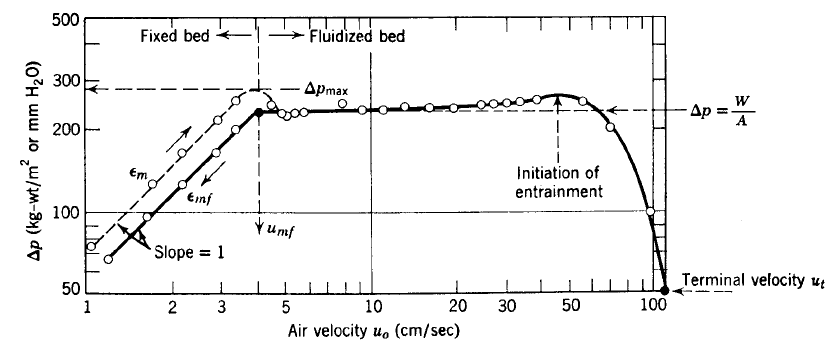
\includegraphics[width=0.6\linewidth]{pressure_drop_vel.png}
%     \caption{Relationship between pressure drop and inlet gas velocity, highlighting the transition from fixed to fluidized bed. Adapted from \cite{pressureDrop}.}
%     \label{fig:pressure_drop}
% \end{figure}

% \subsection{Flow Regime Map}
% To predict the operating state of the reactor based on particle properties and flow conditions, flow regime maps are utilized \cite{flowRegime}. Figure \ref{fig:fluidizeDiagram} presents such a diagram, relating the dimensionless particle diameter $d_p^*$ to the dimensionless gas velocity $u^*$:

% \begin{equation}
%     d_p^* = d_p \sqrt[3]{\dfrac{\rho_f g (\rho_p - \rho_f)}{\eta_c^2}}, \quad
%     u^* = u_f \sqrt[3]{\dfrac{\rho_f^2}{\eta_c (\rho_p - \rho_f) g}}   
% \end{equation}

% where $\eta_c$ represents the dynamic viscosity. This map aids in identifying the boundaries between regimes and determining the optimal operating window—typically between the minimum fluidization velocity and the terminal free-fall velocity—to minimize particle carry-over.

% \begin{figure}[h!]
%     \centering
%     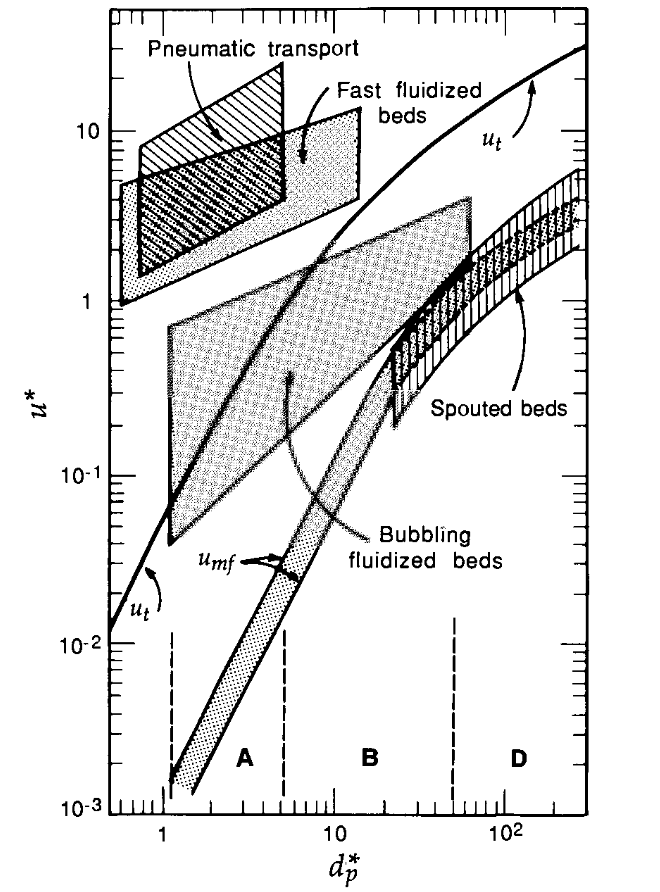
\includegraphics[width=0.5\linewidth]{sections/background/zustand_englisch.png}
%     \caption{Fluidization regime diagram plotting dimensionless velocity against dimensionless particle diameter. Adapted from \cite{zustand_eng}.}
%     \label{fig:fluidizeDiagram}
% \end{figure}



\color{black}
\section{Fluidized Bed Reactor}
\label{sec:basicFBR}
%\Todo{Add image of FBR}
When using iron as a carbon-free energy carrier, both reaction steps, the oxidation and the reduction, need to be as efficient as possible.
Currently, further studies are needed to determine which reactor type gives the most promising results for iron oxide reduction \cite{StudyForReactorNecessary}.
Recent experiments have shown the possibility of reducing iron oxide via a fluidized bed reactor \cite{Malte}. \todo{check bitte nochmal obs inhaltlich so passt}
% A sketch of the used reactor is shown in the following fig \ref{fig:malteFBR}.
% \begin{figure}[h!]
%     \centering
%     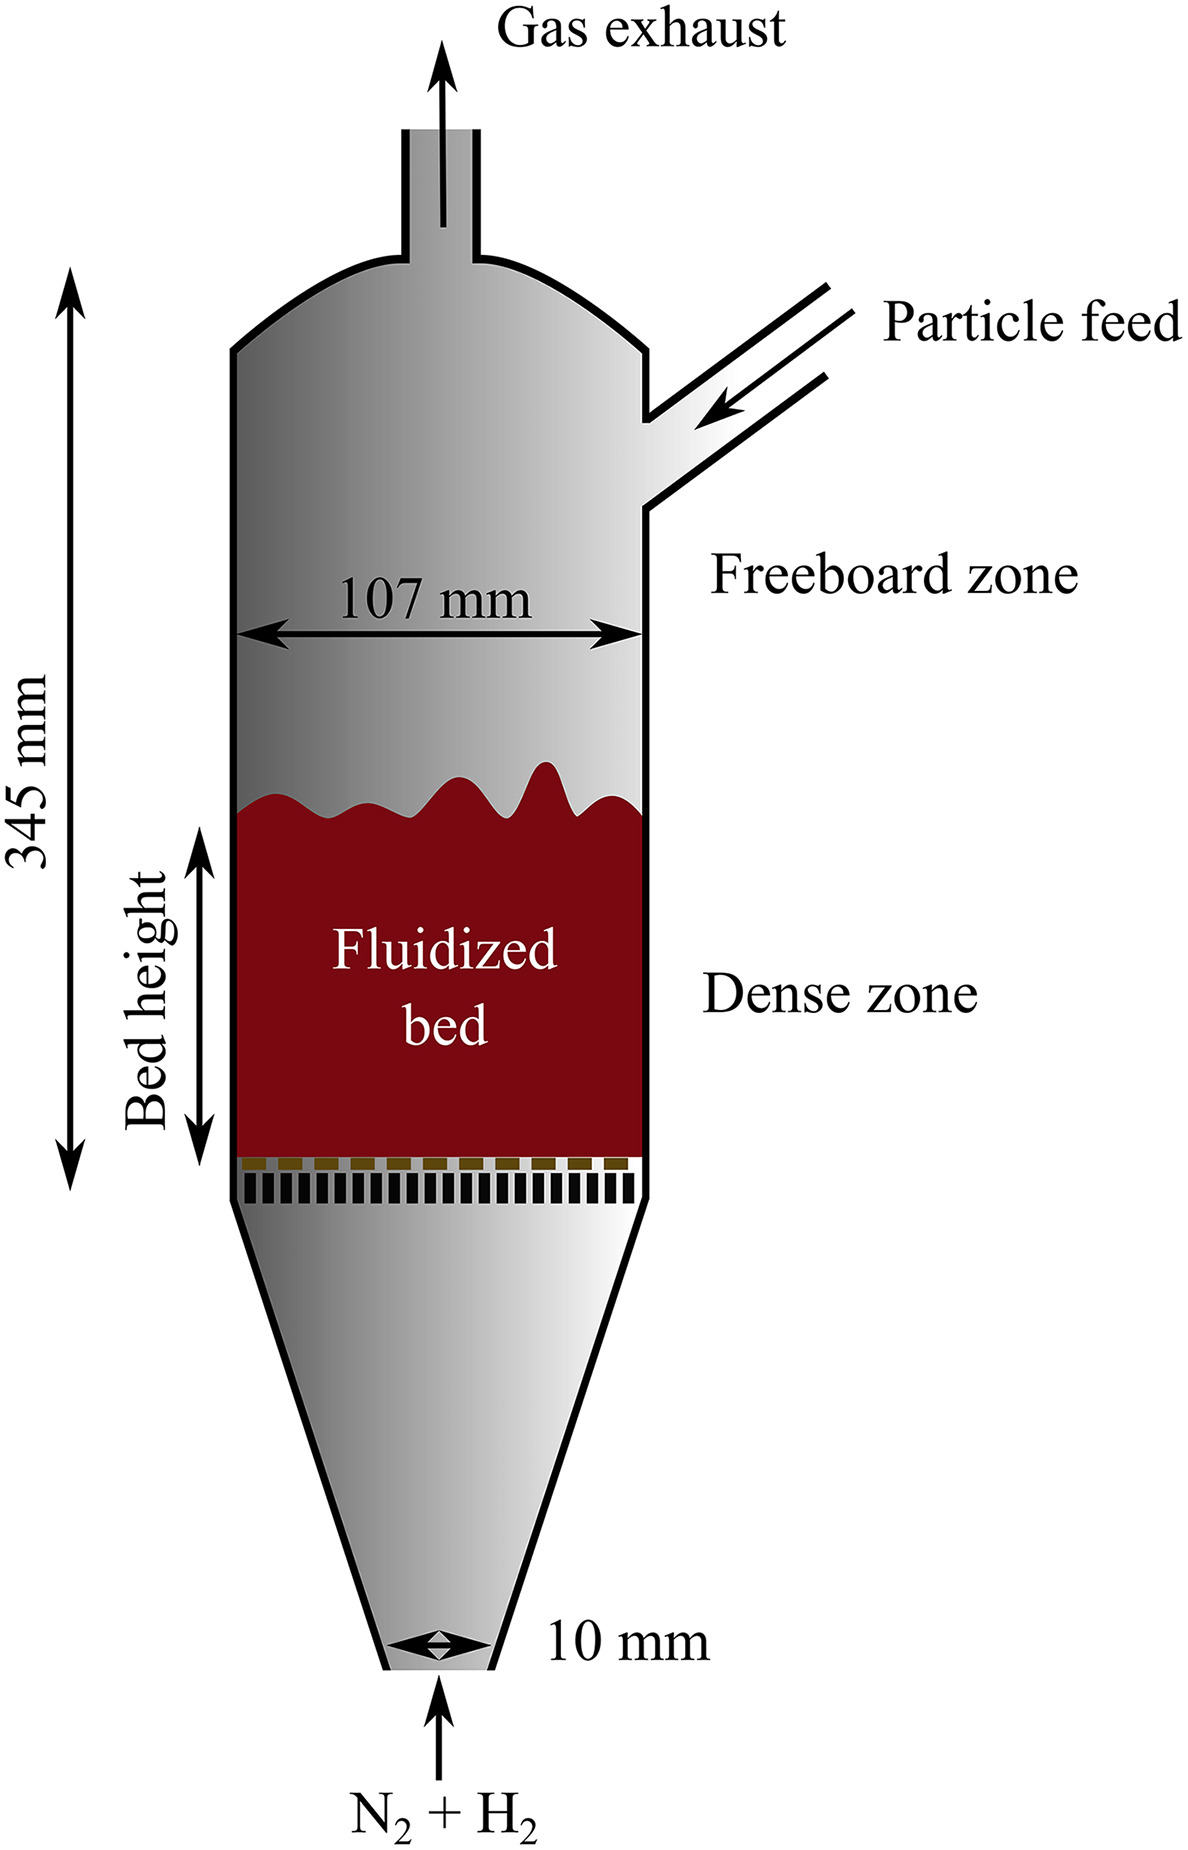
\includegraphics[width=0.3\linewidth]{sections/background/1-s2.0-S0016236125021477-gr3_lrg.jpg}
%     \caption{Caption}
%     \label{fig:malteFBR}
% \end{figure}
In a fluidized bed reactor solid particles are in suspended by an upward flowing fluid, in our case a reducing gas.
This induces fluid-like properties in the particles, such as the ability to maintain a horizontal surface when the reactor is tilted \cite{zustand_eng}.
Due to the suspension of the particles and the rapid mixing, near-isothermal conditions are achieved throughout the reactor and heat and mass transfer between gas and particles are high \cite{advantageFBR}.
%The particles are suspended by the upward flow of the gas.
% Beyond this point, the particles are suspended by the upward flow of the gas and the bed exhibits fluid-like behavior.
%A dense-phase fluidized bed, a bed in which the surface of the bed is still fairly observable, behaves like a fluid.

Particles are either inserted into the reactor via a chute or placed inside the reactor on top of a porous plate. The accumulated particles are called a bed of particles. \todo{vllt particle bed statt bed of particles}
%The particles are suspended by an upward-flowing fluid, in our case gas, causing the particles to behave like a fluid. 
Depending on the gas inlet velocity, the bed shows different behaviors \cite{zustand_eng}.
In fig. \ref{fig:fluidize_states} the different fluidization regimes in a fluidized bed reactor are illustrated.
On the left, the gas inflow rate is low. The gas percolates through the empty spaces in-between the particles. The particles form a fixed bed and remain stationary.
As the flow rate increases, the bed begins to expand.
In the second illustration, the inflow velocity is increased up to the minimum fluidization velocity $\u_{mf}$, where the upward drag force equals the gravitational force on the bed.
%Depending on the inflowing gas velocity different and properties of the solid particles the behavior of the bed varies.
At higher flow rates, the bed does not expand much beyond its minimum fluidization volume. Large instabilities and bubbles start to form, leading to a bubbling fluidized bed.
Bubbles form at the bottom of the bed and coalesce into larger bubbles.
When further increasing the gas velocity, an upper surface of the bed can no longer be observed.
The bed exhibits a turbulent motion and a turbulent fluidized bed is formed.
For even higher velocities, we reach the terminal velocity at which, for a single particle, forces acting on the particle, e.g. drag and gravitational force, are balanced. Exceeding this velocity can lead to particles leaving the reactor.\todo{wenn forces balanced dann solltest du 2 nennen, mein vorschlag: gravitation}
\begin{figure}[h!]
    \centering
    % Each subfigure occupies 24% of the line width
    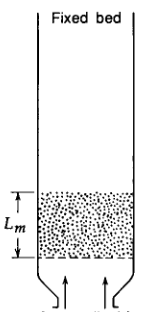
\includegraphics[width=0.24\linewidth,height=8cm, width = 3.5cm,keepaspectratio=false,trim={0 0.1cm 0 0},clip]{sections/background/FixedBed.png}
    \hfill
    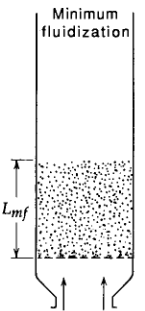
\includegraphics[width=0.24\linewidth,height=8cm,width = 3.5cm,keepaspectratio=false]{sections/background/MinimumFluidization.png}
    \hfill
    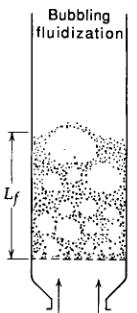
\includegraphics[width=0.24\linewidth,height=8cm,width = 3.5cm, keepaspectratio=false]{sections/background/BubblingFluidization.png}
    \hfill
    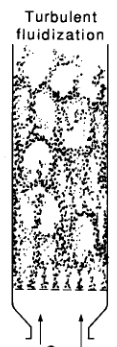
\includegraphics[width=0.24\linewidth,height=8cm,width = 3cm, keepaspectratio=false,trim={0 0.1cm 0 0},clip]{sections/background/TrubulentFluidization.png}
    \caption{Fluidization states in a fluidized bed reactor for different inflow velocities. Inflow velocity increasing from left to right. \cite{zustand_eng}.}
    \label{fig:fluidize_states}
\end{figure}
%\todo{Beim zitieren noch Figure number aus dem Buch angeben?}

% The first is the velocity minimum fluidization velocity $\umf$.
% At the minimum fluidization velocity the drag force exhibited by the upward moving gas is at equilibrium with the weight of the particles.
% The drag force $F_D$ can be expressed as the pressure drop $\Delta \p$ across the bed times the cross section of the reactor $A_r$
% \begin{equation*}
%     F_D = \Delta \p A_r.
% \end{equation*}
% For the weight of the particles we use the volume fraction, the volume of the bed and the specific weight of solids $\gamma = \rho \g$
% \begin{equation*}
%     F_{m_{mf}} = A_r L_{mf} \pvf_{mf} ((\rp - \rf) \g).
% \end{equation*}
% %smaller particles -> higher pressure drop (trade off)
% Equating both forces, we can calculate a ratio of pressure drop to the bed height at minimum fluidization height
% \begin{equation}
% \label{eq:prDrop}
%     \dfrac{\Delta \p}{L_{mf}} = \pvf \Delta \rho \g.
% \end{equation}
% Assuming that the pressure of the particles dominates the pressure difference, $\rp \gg \rf$ we can estimate the pressure drop at minimum fluidization velocity by
% \begin{equation*}
%     \Delta \p \approx \pvf L_{mf} \rp g = \dfrac{\m \g}{A_r}.
% \end{equation*}

To characterize the different states experimentally, we can look at the pressure drop in fig. \ref{fig:presDropRegime}. \todo{mir ist unklar wozwischen der druck gemessen wird, siehe notiz caption bild}
Up to the minimum fluidization velocity, the pressure drop grows approximately linearly. 
At the transition from a fixed bed to a fluidized bed, the pressure drop can increase slightly until the adhesive forces of the particles are overcome.
Above the minimum fluidization velocity, the pressure drop stays nearly constant. 
After reaching the terminal velocity, the pressure drop decreases.
\begin{figure}[h!]
    \centering
    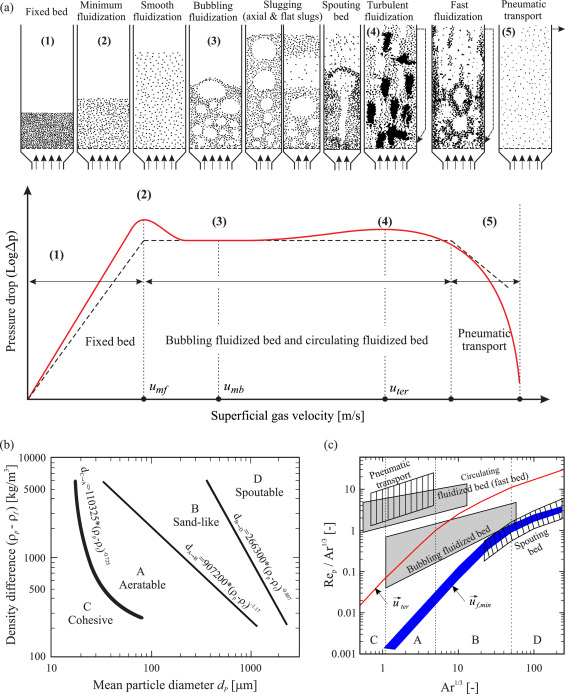
\includegraphics[width=0.8\linewidth, trim = {0cm 6cm 0cm 4cm},clip]{sections/background/1-s2.0-S0360128521000289-gr2.jpg}
    \caption{Pressure drop for different inlet gas velocity \cite{feichi}. }
    \label{fig:presDropRegime}
\end{figure}
\todo{Oder erkläre in der caption genauer was für ein pressure drop es ist}

%https://link.springer.com/article/10.1007/s13399-020-01189-9 explains going up or down

%uO superficial gas velocity *measured on an empty vessel basis) through a bed of solids

% The pressure drop increases linearly with a inlet velocity below the minimum fluidization velocity. 
% \Todo{Ergun equation}

To predict the operating state of our bed in the reactor, we can use a flow regime map for gas-solids fluidization \cite{flowRegime}.
\begin{figure}[h!]
    \centering
    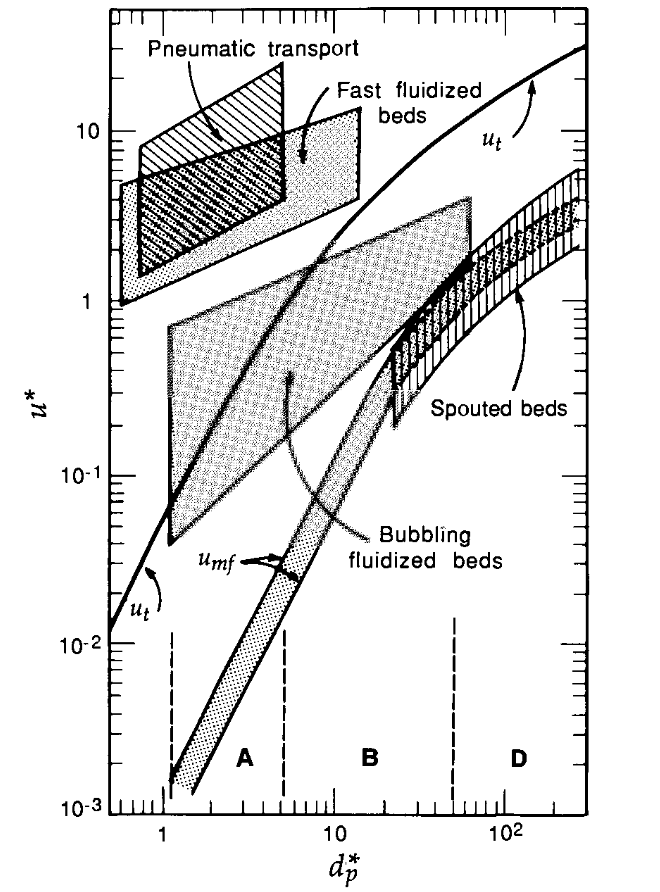
\includegraphics[width=0.5\linewidth]{sections/background/zustand_englisch.png}
    \caption{Fluidization regime diagram for the dimensionless particle parameter and inlet velocity. From: \cite{zustand_eng}}
    \label{fig:fluidizeDiagram}
\end{figure}
\todo{ich weiß nicht wie genau ihr über Quellenangaben gesprochen habt, shota hätte das hier nicht gerreicht, sondern da müsste die genaue seite stehen oder weitere details}
The diagram in figure \ref{fig:fluidizeDiagram} relates the dimensionless particle diameter 
\begin{equation*}
 d_p^* = d_p \sqrt[3]{\dfrac{\rf \g \Delta \rho}{\eta_c^2}}.
\end{equation*}
on the $x$-axis to the dimensionless gas velocities
\begin{equation*}
u^* = \uf \sqrt[3]{\dfrac{\rf^2}{\eta_c \Delta\rho \g}}    
\end{equation*}
on the $y$-axis and classifies different fluidization regimes. Here $d_p$ is the particle diameter, $\uf$ is the fluid velocity, $\rf$ is the gas density, $g$ is the gravitational force, $\Delta \rho$ is the difference between the solid and gas density and $\eta_c$ is the kinematic gas viscosity.
The diagram aids in distinguishing between the different fluidization regimes.
We can see that bubbling fluidized beds are achieved for velocities above the minimum fluidization velocity. For larger particles, the gap in dimensionless velocity between the two decreases.
The terminal velocity for smaller particles coincides with the bubbling fluidized bed. 


% Two empirically calculated velocities are shown. The first is the minimal fluidization velocity discussed earlier.
% It is based on the empirical correlation by Ergun \cite{Ergun} for the pressure drop
% \begin{equation*}
%     \dfrac{\Delta \p}{L} = 150 \dfrac{\nu (1-\fvf_{mf})^2}{\fvf_{mf}^3 d_{32}^2} \umf + 1.75 \dfrac{(1-\fvf_{mf}) \rf}{\fvf_{mf}^3 d_{32}} \umf^2
% \end{equation*}
% where we choose $150$ and $1.75$ as constants.
% Here the first term represents the viscous energy loss and the second term the inertial loss \cite{ErgExp}.
% We combine these with equation \eqref{eq:prDrop} for the dimensionless form
% \begin{equation*}
%     \dfrac{1.75}{\fvf_{mf}^3 \phi_s} \operatorname{Re}^2_{p,mf} + \dfrac{150 (1-\fvf_{mf})}{\fvf_{mf}^3 \phi_s^2} \operatorname{Re}_{p,mf} = \operatorname{Ar} \qquad \operatorname{Ar} = \dfrac{d_p^3 \rf (\rp - \rf) \g}{\mu ^2} \quad \operatorname{Re}_{p,mf} = \dfrac{\rf d_p \umf}{\mu}.
% \end{equation*}
% which we simplify to
% \begin{equation*}
%     \operatorname{Ar} = K_1 \operatorname{Re}_{p,mf} + K_2 \operatorname{Re}^2_{p,mf}.
% \end{equation*}
% Here $\operatorname{Ar}$ is the Archimedes number, also sometimes known as Galileo number, e.g. \cite{predictWenYu}, which describes the motion based on the density difference and $\operatorname{Re}_{p,mf}$ is the particle Reynolds number.
% A simplification of the term for fine particles was proposed by Wen and Yu \cite{WenYu} 
% \begin{equation*}
%     \dfrac{(1-\fvf_{mf})}{d_{32}^2 \fvf_{mf}^3} \approx 11 \quad \dfrac{1}{d_{32} \fvf_{mf}^3} \approx 14 \qquad \operatorname{Re}_{mf} = \sqrt{(33.7)^2 + 0.0408 \operatorname{Ar}} - 33.7
% \end{equation*}
% which is reasonable at room temperature.
% Although the author claim that the approximation covers a diameter range of $[0.002,1.97]$ and a minimum fluidization velocity of $[0.136,1.0]$.
% Solving for the $d_{32}$ and $\fvf_{mf}$ we can see that the equation only hold for $\fvf_{mf} = 0.47, 0.93$ and $\d_{32} = 0.67, 0.09$.


% Apart from the minimum fluidization velocity we can also calculate the terminal free-fall velocity. This represents a equilibrium of the gravitational force, 
% Keeping the velocity above $\umf$ and below $\u_t$ reduces carry over of particles from a fluidized bed.
% To calculate $\u_t$ we use the diameter of the smallest particles 
% \begin{equation*}
%     \u_t = \left[ \dfrac{4 d_{p,s} (\rp - \rf)\g}{3 \rf C_D}\right]^{1/2}
% \end{equation*}
% and the experimentally determined drag coefficient given by \cite{Haider} and \cite{TURTON1987127} we get the terminal velocity
% \begin{align*}
%     \u_t^* = 
%     \begin{cases}
%         \left( \dfrac{18}{d_p^*)^2} + \dfrac{2.335 - 1.744 \phi}{(d_p^*)^{0.5}} \right)^{-1}, & 0.5 < \phi < 1 \\
%         \left( \dfrac{18}{(d_p^*)^2} + \dfrac{0.591}{(d_p^*)^{0.5}} \right)^{-1}, & \phi = 1.
%     \end{cases}
% \end{align*}

% \todo{Relevanz irgendwie nicht ganz gegeben...}




% The properties of the solid particles strongly influence the fluidization behavior.


% diameter of the particles $d_p$, or the diameter distribution, the density difference between the fluid and the particles $\Delta \rho = \rp / \rf$. From these factors we can calculate the dimensionless particle diameter
% \begin{equation*}
%  d_p^* = d_p \sqrt[3]{\dfrac{\rf \g \Delta \rho}{\eta_g^2}}.
% \end{equation*}
% In the following diagram \ref{fig:fluidizeDiagram} we can then determine the corresponding dimensionless velocities
% \begin{equation*}
% u^* = \uf \sqrt[3]{\dfrac{\rf^2}{\eta_g \Delta\rho \g}}    
% \end{equation*}


% The four boundaries he suggested are as
% follows:
% 56 Yang
% Group C boundary
% G roup A/C boundary
% G roup A/B boundary
% G roup B/D boundary
% Ar = 0.97
% Ar = 9.8
% Ar = 88.5
% Ar = 176,900
% (12)
% (13)
% (14)
% (15)


% \begin{itemize}
%     \item fluid (in our case gas) passed through a solid granular material at high enough speeds to suspend the solid and cause it to behave as though it were a fluid (fluidization)
%     \item supported by a porous plate (distributor)
%     \item At lower fluid velocities, the solids remain in place as the fluid passes through the voids in the material. This is known as a packed bed reactor.
%     \item As the fluid velocity is increased, the reactor will reach a stage where the force of the fluid on the solids is enough to balance the weight of the solid material. This stage is known as incipient fluidization and occurs at this minimum fluidization velocity. 
%     \item Once this minimum velocity is surpassed, the contents of the reactor bed begin to expand and swirl around much like an agitated tank or boiling pot of water. The reactor is now a fluidized bed. Depending on the operating conditions and properties of solid phase various flow regimes can be observed in this reactor. 
%     \item advantages:
%     \begin{itemize}
%         \item The high gas flow results in an efficient contact between the reactants and the catalysts, leading to the enhanced heat and mass transfer rates on the catalyst surfaces. As a result, the non-uniform temperature distribution that commonly exists in fixed-bed reactor could be avoided. (https://www.sciencedirect.com/science/article/pii/S136403211930797X)
%         \item
%     \end{itemize}
% \end{itemize}




% The behavior of particles being suspended by inflow of gas differs wildly.
% For small fluid velocities, the gas goes through spaces between the particles. Increasing the fluid velocity particles start to be carried upward by the fluid leading to bubbles. Coalescence forces lead to bubbles increasing in size. For larger fluid velocities the bubble diameter can increase to the diameter of the column.


% A rough categorization, for increasing fluid velocity, is depicted in figure \ref{fig:fluidize_states}.

% \begin{figure}
%     \centering
%     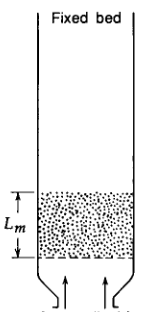
\includegraphics[width=0.24\linewidth,trim = {0 0.1cm 0 0}, clip]{sections/background/FixedBed.png}
%     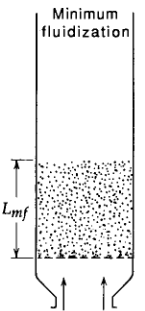
\includegraphics[width = 0.24\linewidth]{sections/background/MinimumFluidization.png}
%     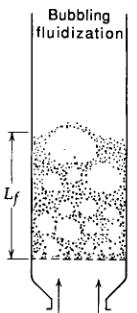
\includegraphics[width = 0.24 \linewidth]{sections/background/BubblingFluidization.png}
%     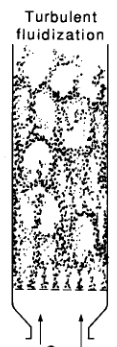
\includegraphics[width = 0.24 \linewidth, trim = {0 0.1cm 0 0}, clip]{sections/background/TrubulentFluidization.png}
%     \caption{Caption}
%     \label{fig:fluidize_states}
% \end{figure}




% \begin{figure}[h!]
%     \centering
%     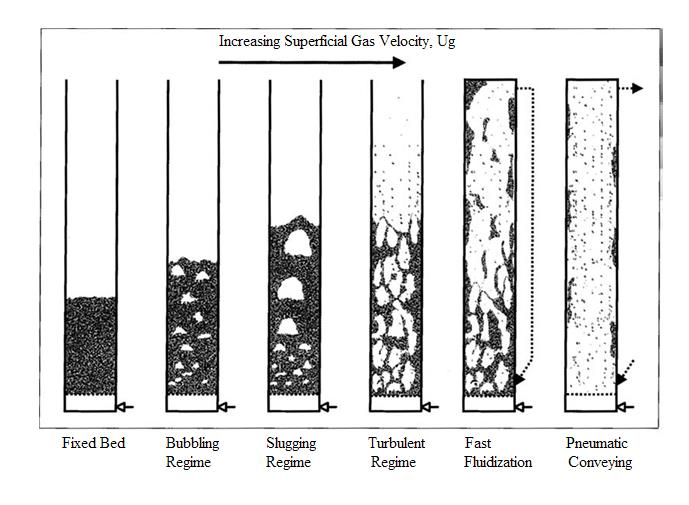
\includegraphics[width=0.8\linewidth]{Fluidization-regimes-in-a-gas-solid-fluidized-bed-Crowe-2006.png}
%     \caption{Fluidization regimes for increasing gas velocities. From }
%     \label{fig:fluidize_states}
% \end{figure}





% \section{Modelling of Gas-Solid Systems}
% \label{sec:modelling_intro}

% Before simulating a fluidized bed reactor, it is essential to understand the fundamental approaches to modeling multiphase systems in Computational Fluid Dynamics (CFD) \cite{cfdComp}.
% In gas-solid flows, the gas phase is almost exclusively modeled as a **continuous phase** (Eulerian framework). In this approach, the fluid is treated as a continuum where macroscopic properties---such as density, velocity, and pressure---are defined as fields averaged over computational cells.

% The **solid phase**, however, can be represented in two distinct ways:
% \begin{enumerate}
%     \item \textbf{Discrete Phase (Lagrangian):} The solid material is treated as distinct, individual entities (particles). The motion of each particle is tracked by solving Newton’s equations of motion. This preserves the discrete nature of the solids, including their history and trajectories.
%     \item \textbf{Continuous Phase (Eulerian):} The solid phase is treated as a "pseudo-fluid" interpenetrating the gas phase. Particle properties are averaged over control volumes, converting discrete mass into a continuous density field.
% \end{enumerate}

% These representations lead to different numerical methods, primarily distinguished by how they handle particle-particle interactions.

% \subsection{Discrete Particle Methods (Euler-Lagrange)}
% Using a solver with a fully discrete solid phase, such as the Discrete Element Method (DEM) or the discrete parcel method in \OF, allows for the precise resolution of granular dynamics.
% In these methods, every collision and contact force between particles is explicitly calculated. While highly accurate, the computational cost is significant. The simulation time typically scales non-linearly with the number of particles (often $N \log N$ or $N^2$ depending on the neighbor-search algorithm). Consequently, this approach is often computationally prohibitive for industrial-scale applications containing millions of particles.

% \subsection{Continuum Methods (Euler-Euler)}
% To simulate larger systems, the solid phase can be modeled as a continuum using the Two-Fluid Model (TFM).
% In this Euler-Euler approach, particle-particle interactions are not resolved individually but are instead modeled through closure relations (e.g., Kinetic Theory of Granular Flow).
% While this method is computationally efficient, the averaging process smoothes out discrete flow structures. This can lead to inaccuracies, particularly in regimes with sharp interfaces or complex particle size distributions \cite{mathMPPIC}.

% \subsection{The Hybrid Approach: MP-PIC}
% To mitigate the high computational cost of discrete methods while retaining the accuracy of Lagrangian tracking, we utilize the Multiphase Particle-in-Cell (\MP) method.
% This is a hybrid approach in which the gas is continuous (Eulerian) and the solids are discrete (Lagrangian), but particle-particle interactions are handled via a continuum approximation.
% Instead of resolving individual collisions, the \MP method maps particle properties to the Eulerian grid to calculate a "particle normal stress" gradient. This gradient is then interpolated back to the particles to apply a repulsive force, mimicking the effect of collisions without the expensive contact detection.

% In the \MP method, interpolation operators are used to transfer properties between the discrete parcels and the continuous grid.
% The primary advantage is that interaction forces are calculated from gradients on the Eulerian grid, meaning the computational cost scales linearly with the number of particles ($O(N)$), rather than quadratically.
% The theoretical derivation of the \MP method is detailed in Chapter \ref{ch:MPPIC}, followed by its implementation in \OF in Chapter \ref{ch:OpenFOAM}.







\section{Modelling of Gas-Solid Systems}
Before we simulate a fluidized bed reactor, we first look at how multiphase systems are generally modeled in CFD \cite{cfdComp}.
We have two phases we need to model for our fluidized bed reactor, the fluid phase (gas) and the dispersed solid phase (particles).
The fluid is generally treated as a continuum, therefore its properties, such as volume fraction, pressure and velocity, are modeled by continuous fields. 
The dispersed phase as shown in fig. \ref{fig:solidClass} can be modeled using one of two main approaches.
\FloatBarrier
\begin{figure}[h!]
\centering
    \begin{tikzpicture}[
  sibling distance=6em,
  level distance=4em,
  every node/.style = {font=\normalsize},
  edge from parent/.style = {draw, -latex},
  level 1/.style={sibling distance=12.5em},
  level 2/.style={sibling distance=8em},
  highlight/.style={draw=kit-red, very thick}, opacity = 1%ellipse, inner sep=2pt}
  ]

\node[align = center, auto = right, near end]{Solid phase\\representation}
  child {node[align = center, auto = right, near end] {Discrete}
    %child {node[align = center, auto = right, near end] (leftroot){Particle Resolved\\Direct Numerical\\Simulations\\PR-DNS}}
    child {node[align = center, auto = right, near end] (leftroot){Discrete Particle Model\\DPM}}
  }
  child {node[align = center, auto = right, near end] {Hybrid Models}
  child {node[align = center, auto = right, near end, highlight] {Multiphase-Particle-In-Cell \\ MPPIC}}}
  child {node[align = center, auto = right, near end] {Continuum}
    child {node[align = center, auto = right, near end] (rightmost){Two Fluid Model\\ twoPhaseEuler}}
    % child  {node[align = center, auto = right, near end] (rightmost) {Mixture Model\\MM}}
  };
  \draw[->, thick]
  ([yshift=-48pt]leftroot.west) --
  ([yshift=-48pt]rightmost.east |- leftroot.west)
  node[midway, above] {computationally less expensive};
  \draw[->, thick]
  ([yshift=-60pt]rightmost.east |- leftroot.west) --
  ([yshift=-60pt]leftroot.west)  
  node[midway, below] {more accurate};
\end{tikzpicture}
\caption{Classification of solvers based on the representation of the solid phase. Adapted from: \cite{mathMPPIC}.}
\label{fig:solidClass}
\end{figure}
\FloatBarrier
In the continuum approach, the particulate phase is treated analogously to the fluid phase. Transport equations are solved for average quantities such as velocity and fluid fraction.
Particle-particle interactions, like collisions, are considered indirectly, often through a solid stress tensor.
Conservation equations are obtained through volume averaging. The two phases are coupled via the phase volume fractions.
In \OFns, simulations are run with the \lstinline|twoPhaseEulerFoam| solver.
Although this model is computationally less expensive, the modeling used requires closure relations. Generally, more closure relations lead to lower model accuracy but also reduced computation time \cite{mathMPPIC}.
On the other hand, we can model particles as a discrete phase, which is more suitable for dense particulate flows.
%In a fluidized bed reactor particle-particle interactions are significant. 
Here, each particle, along with properties like velocity and mass, is tracked individually and in \OF each particle-particle interaction is resolved via a spring-dashpot model. This method is computationally expensive and scales exponentially with the number of particles.
To mitigate the disadvantages of both methods, we use a hybrid model, called the Multiphase-Particle-In-Cell (\MPns) method.
Particle trajectories are advanced as dispersed particles, with each being tracked individually. After they are moved, the positions are interpolated and treated as a continuous phase. 
The continuous properties of both phases are then calculated based on the continuous fields. The continuous properties are interpolated back to the particles and used to calculate the next time step.
The acceleration of the particles due to collisions is calculated as in the Euler-Euler method by using a solid stress tensor.




% The fluid is generally modeled as a continuum, therefor with properties like, volume fraction, density, pressure and velocity as continuous functions of space and time.
% For the particles we can use one of two main approaches. 
% First we could model them as a continuous phase, coupling the particles through a phase fraction for each cell to the fluid phase.
% Here particle-particle interactions, like collision are modeled through the solid stress tensor.
% Conservation equations are obtained through averaging methods.
% To mitigate the disadvantages from the previously mentioned methods we will use a hybrid approach which models particle as a discrete phase but models interactions through the particle normal stress and damping terms without resolving them, called the Multiphase-Particle-In-Cell (\MP\hspace{-12pt}) method.

\color{black}

% In this method the particles are modeled as both a discrete and a continuous phase with interpolation operators being used to transfer properties between the two.
% The main advantage of this method is, that particle-particle interactions are calculated from parameters that only depend on the Eulerian grid and are not fully resolved.
We will discuss in detail how the \MP method works by first looking at the paper that presented the method in ch. \ref{ch:MPPIC} and then at the \OF implementation discussed in ch. \ref{ch:OpenFOAM}.
%twoPhaseEuler: https://www.tfd.chalmers.se/~hani/kurser/OS_CFD_2014/Alessandro%20Manni/ReportAM.pdf




% Our main goal is to simulate a fluidized bed reactor. In the \OF tutorials folder, a fluidized bed is pre-implemented with two different solvers. 
% The first solver is called \DP and tracks each particle and models their collisions. 
% Modeling each particle and collision requires a high computational effort.
% Therefor in this chapter we will look at the \MP solver which mitigates the complexity by modeling particle interactions through the particle normal stress on the Eulerian grid.
% On top of that particles can be grouped into parcels with similar characteristics, reducing computation time further. 
% The first one gives a more accurate solution while the latter has a lower computational effort which is useful when the trend of the experiment is more important than the accuracy.
% \color{gray}
% \section{Overview of Gas-Solid Multiphase Flow Solvers}
% Our goal of this section is to look at a brief overview of different CFD approaches. 
% These approaches can be roughly divided into two categories: The Euler-Euler methods and the Euler-Lagrange methods. 
% The Eulerian-Eulerian methods model both the gas and the solid phase as a continuum. In the Euler-Lagrange model the gas is modeled as a continuous phase and the solid as a discrete phase.
% The \MP-model is a hybrid model, constructed in a way that exploits the advantages of both the Euler-Euler method as well as the Euler-Lagrange method.


%\Todo{EE und EL erklären? Welche alles?} 

% \begin{itemize}
%     \item something about Euler-Euler and Euler-Lagrange
%     \item OpenFoams DPMFoam is not the logical Lagrangian Disecrete Phase Model (which has no collision) but brobably DDPM-KTGF (Dense Discrete Phase Model incorporated with Kinetic Theory of Granular Flow)
% \end{itemize}
